\documentclass[
  bibliography=totoc,     % Literatur im Inhaltsverzeichnis
  captions=tableheading,  % Tabellenüberschriften
  titlepage=firstiscover, % Titelseite ist Deckblatt
]{scrartcl}

% Paket float verbessern
\usepackage{scrhack}

% Warnung, falls nochmal kompiliert werden muss
\usepackage[aux]{rerunfilecheck}

% unverzichtbare Mathe-Befehle
\usepackage{amsmath}
% viele Mathe-Symbole
\usepackage{amssymb}
% Erweiterungen für amsmath
\usepackage{mathtools}

% Fonteinstellungen
\usepackage{fontspec}
% Latin Modern Fonts werden automatisch geladen
% Alternativ zum Beispiel:
%\setromanfont{Libertinus Serif}
%\setsansfont{Libertinus Sans}
%\setmonofont{Libertinus Mono}

% Wenn man andere Schriftarten gesetzt hat,
% sollte man das Seiten-Layout neu berechnen lassen
\recalctypearea{}

% deutsche Spracheinstellungen
\usepackage[main=ngerman]{babel}


\usepackage[
  math-style=ISO,    % ┐
  bold-style=ISO,    % │
  sans-style=italic, % │ ISO-Standard folgen
  nabla=upright,     % │
  partial=upright,   % ┘
  warnings-off={           % ┐
    mathtools-colon,       % │ unnötige Warnungen ausschalten
    mathtools-overbracket, % │
  },                       % ┘
]{unicode-math}

% traditionelle Fonts für Mathematik
\setmathfont{Latin Modern Math}
% Alternativ zum Beispiel:
%\setmathfont{Libertinus Math}

\setmathfont{XITS Math}[range={scr, bfscr}]
\setmathfont{XITS Math}[range={cal, bfcal}, StylisticSet=1]

% Zahlen und Einheiten
\usepackage[
  locale=DE,                   % deutsche Einstellungen
  separate-uncertainty=true,   % immer Fehler mit \pm
  per-mode=symbol-or-fraction, % / in inline math, fraction in display math
]{siunitx}

% chemische Formeln
\usepackage[
  version=4,
  math-greek=default, % ┐ mit unicode-math zusammenarbeiten
  text-greek=default, % ┘
]{mhchem}

% richtige Anführungszeichen
\usepackage[autostyle]{csquotes}

% schöne Brüche im Text
\usepackage{xfrac}

% Standardplatzierung für Floats einstellen
\usepackage{float}
\floatplacement{figure}{htbp}
\floatplacement{table}{htbp}

% Floats innerhalb einer Section halten
\usepackage[
  section, % Floats innerhalb der Section halten
  below,   % unterhalb der Section aber auf der selben Seite ist ok
]{placeins}

% Seite drehen für breite Tabellen: landscape Umgebung
\usepackage{pdflscape}

% Captions schöner machen.
\usepackage[
  labelfont=bf,        % Tabelle x: Abbildung y: ist jetzt fett
  font=small,          % Schrift etwas kleiner als Dokument
  width=0.9\textwidth, % maximale Breite einer Caption schmaler
]{caption}
% subfigure, subtable, subref
\usepackage{subcaption}


% Grafiken können eingebunden werden
\usepackage{graphicx}
% größere Variation von Dateinamen möglich
%\usepackage{grffile}

% schöne Tabellen
\usepackage{booktabs}

% Verbesserungen am Schriftbild
\usepackage{microtype}
\setlength{\parindent}{0pt}

% Literaturverzeichnis
\usepackage[
  backend=biber,
]{biblatex}
% Quellendatenbank
\addbibresource{lit.bib}
\addbibresource{programme.bib}

% Hyperlinks im Dokument
\usepackage[
  german,
  unicode,        % Unicode in PDF-Attributen erlauben
  pdfusetitle,    % Titel, Autoren und Datum als PDF-Attribute
  pdfcreator={},  % ┐ PDF-Attribute säubern
  pdfproducer={}, % ┘
]{hyperref}
% erweiterte Bookmarks im PDF
\usepackage{bookmark}

% Trennung von Wörtern mit Strichen
\usepackage[shortcuts]{extdash}

% Import PDFs
\usepackage{pdfpages}


\usepackage{graphicx}

% Chemische Notation mit Kernladung und masse
\usepackage{isotope}
% definiert Befehl \isotope[A][B]{X}
% und $\isotope[6][3]{Li}+\isotope[2][1]{H} \to\isotope[4][2]{He}+\isotope[4][2]{He}$ Beispiel






\title{Lebensdauer kosmischer Myonen\\
\small{Versuch 01}
}
\author{%
  Marcel Kebekus\\%
  \href{mailto:marcel.kebekus@tu-dortmund.de}{marcel.kebekus@tu-dortmund.de} \and
  Konstantin Mrozik\\
  \href{mailto:konstantin.mrozik@tu-dortmund.de}{konstantin.mrozik@tu-dortmund.de}%
}
\date{
  Abgabe: \today %??????????
}
\publishers{TU Dortmund – Fakultät Physik}
\makeatletter         
\def\@maketitle{
\raggedright

\includegraphics[width=\textwidth]{bilder/lo_TU-Do_2008/logo_rgb_jpg/tud_logo_rgb.jpg}\\[8ex]
\begin{center}
{\Huge \bfseries \sffamily \@title }\\[4ex] 
{\Large  \@author}\\[4ex] 
\@date\\[8ex]
\publishers\\
\end{center}}
\makeatother


\begin{document}


\maketitle
\thispagestyle{empty}
\tableofcontents
\newpage
\section{Ziel}
Ziel ist die Durchführung von akustischen Experimenten mit einem Kugelresonator und verschiedenen Resonatorketten
sowie der Vergleich mit quantenmechanischen Systemen eines Wasserstoffatoms, Wasserstoffmoleküls und 1-dimensionalen Festkörpern.

\section{Versuchseinführung}
Im Folgenden Versuch wird mithilfe eines Mikrofons und eines Lautsprechers die Druckverteilung in einem Rohr- und Kugelresonator 
betrachtet. Dazu wird jeweils das Frequenzspektrum für die jeweiligen Resonatoren betrachtet, die durch ein Frequenz-zu-Spannung-Konverter
mittels einer geeigneten Software erstellt werden. 

\section{Theorie}
Bei den vermessenden Resonatoren kann ein Vergleich zu quantenmechanischen Modellen gezogen werden. In diesem 
Abschnitt sollen die Gemeinsamkeiten zwischen den im Versuch betrachteten Modellen und ihren
quantenmechanischen Analogien aufgezeigt werden.\\


Die Druckverteilung in einem Resonator kann mithilfe der Helmholtzgleichung
\begin{equation}
    \Delta \varphi=\lambda \cdot \varphi
    \label{eq:helmholtz_all}
\end{equation}
beschrieben werden. Diese Differentialgleichung beschreibt die Druckänderung mit der Von-Neumann-Randbedingung
\begin{equation*}
    v\left(0\right) = v\left(L\right) = 0
\end{equation*}




\subsection{Der Rohrresonator}
Der Rohrresonator wird an einem Ende mit dem Mikrofon und am anderen Ende mit dem Lautsprecher abgeschlossen.
Beim Abspielen einzelner Frequenzen entsteht genau dann eine Resonanz, wenn die Wellenlänge $\lambda$ der Schallwelle
mit der Reflexion der Welle konstruktiv interferiert. Dies geschieht genau dann, wenn gilt
\begin{equation}
    L=n\frac{\lambda}{2}=n\frac{c}{2f}.
\end{equation}
Wobei $L$ die Rohrlänge, $c$ die Schallgeschwindigkeit, $f$ die Frequenz der Schallwelle und $n$ ein ganzzahliges Vielfaches ist.
Im Rohr findet dabei nur eine Ausbreitung der Luftmoleküle mit Ausbreitungsrichtung der Schallwelle statt.
Die Druckverteilung $P(x,t)$ ergibt sich dann mit der Gleichung \ref{eq:helmholtz_all} zu
\begin{equation}
    \frac{\partial^2}{\partial t^2}P(x,t)=\frac{1}{\rho \kappa}\frac{\partial^2}{\partial x^2}P(x,t)
\end{equation}
\label{sec:Theorie}
wobei $\rho$ die Dichte und $\kappa$ die Kompressiblität des Mediums ist in dem sich die Schallwellen ausbreiten (hier: Luft).
Daraus folgt die zeitabhängige Lösung
\begin{equation}
    P(x,t)=p(x)\cdot \cos{(wt)}
    \label{eq:rohr_loe}
\end{equation}
mit dem Ortsanteil $p(x)$.
Die Kreiszahl $k$ lässt sich über die Beziehung $k=2\pi/\lambda$ zu
\begin{equation}
    k=\frac{n\pi}{L}
\end{equation}
bestimmen.

\begin{figure}
    \center
    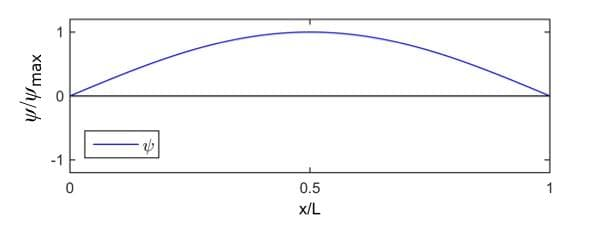
\includegraphics[width=0.7\textwidth]{bilder/Resonanz.jpg}
    \caption{Skizze zur Herleitung der Resonanz im Rohrresonator. Zu sehen ist die Grundschwingung. \cite{uni}}
\end{figure}

\subsubsection{Rohrresonator mit Blenden}
Koppelt man zwei Rohrresonatoren mit einer Blende, so verhält sich das System ähnlich zu einem 
gekoppelten Pendel. Es kommt zur einer zusätzlichen Resonanz $\omega_{R2}$ zur Ursprungsresonanz $\omega_{R1}$.
Es gilt zusätzlich $\omega_{R2}\geq \omega_{R1}$. Dies lässt sich nun durch eine Kette von Resonatoren und Blenden weitertreiben, wobei
jeweils zusätzliche Resonanzen auftreten, die im Spektrum immer dichter aneinander liegen.
Bei unendlich vielen gekoppelten Resonatoren kann man von einem Band sprechen.
Analog zu einem 1-dim-Festkörper kann man hier von einer Bandlücke sprechen.

\subsection{Analogon Teilchen im unendlichen Potenzialtopf}
Der Vergleich mit einem Teilchen im unendlichen Potenzialtopf ist dabei ein Analogon für Materie (bzw. Elektronen und Protonen)mit einem Wellencharakter, welcher durch die de-Broglie-Wellenlänge $\lambda_B$ über
\begin{equation}
    \lambda_B=\frac{h}{p}
\end{equation}
mit dem planckschen Wirkungsquantum $h$ und dem Impuls des Teilchens $p$ beschrieben werden kann.
Die Differentialgleichung für die Wellenfunktion $\Rho(x,t)$ für das Teilchen im Kasten folgt dabei aus der Schrödingergleichung
\begin{equation}
    i\hbar \frac{\partial}{\partial t}\Rho(x,t)=-\frac{\hbar^2}{2m}\frac{\partial^2}{\partial x^2}\Rho(x,t)+V(x)\Rho(x,t)
\end{equation}
mit der Teilchenmasse $m$, dem Potenzial $V(x)$. Für den unendlichen Potenzialtopf gilt $V(0 < x < L)=0$ und
$V(x \geq L)\rightarrow \infty$ und $V(x \leq 0)\rightarrow \infty$.
Damit ergibt sich die Lösung
\begin{equation}
    \Rho(x,t)=\rho(x)\cdot \exp{(-i\omega t)}
\end{equation}
und die zeitunabhängige Schrödingergleichung
\begin{equation}
    E\rho(x)=\frac{\hbar^2}{2m}\frac{\partial^2}{\partial x^2}\rho(x)
\end{equation}
mit der Energie $E$.
Für eine stehende Welle folgt daraus die Gleichung der Form
\begin{equation}
    \rho(x)=A\sin{(kx+\phi)}
    \label{eq:quant_loe}
\end{equation}
mit der komplexen Amplitude $A$, der Kreiszahl $k$ und der Phase $\phi$.
An den Rändern ergibt sich dabei eine Wellenfunktion von null, sodass aus dieser Randbedingung
$\rho(x=0)=0$ und $\rho(x=L)=0$ folgt
\begin{equation}
    k=\frac{n\pi}{L}.
    \label{eq:k}
\end{equation} 

Es wird deutlich das der Vergleich der beiden Modelle berechtigt ist. Im klassischen Fall erzeugt man eine kosinusabhängige stationäre
Druckverteilung (vgl. Gl. \ref{eq:rohr_loe}), während das quantenmechanische Modell 
eine stationäre Wahrscheinlichkeitsverteilung ergibt (vgl. Gl. \ref{eq:quant_loe}). Unterschiede zeigen sich bei den Randbedingungen.
Denn während bei dem quantenmechanischen Teilchen die Wahrscheinlichkeitsdichte verschwindet, sind an den Enden des Rohres 
die Druckunterschiede maximal, was allerdings kein Einfluss auf die erlaubten Wellenlängen hat.
Beide Modelle bilden dabei stehende Wellen für die Kreiszahl $k$ nach Gleichung \ref{eq:k} aus.


\subsection{Der Kugelresonator}
Nun wird ein Resonator mit einer Kugelform betrachtet (Hohlkugel), der aus zwei Halbkugeln besteht, welche gegeneinander verdreht werden können.
Somit können die Resonanzamplituden in Abhängigkeit des Winkels $\alpha$ gemessen werden.

Zur genauen Beschreibung des dreidimensionalen Problems der Druckverteilung wird nun die Kugelsymmetrie mit den Koordinaten des Polarwinkels $\theta$ (0 bis $\pi$)
und des Azimutwinkel $\varphi$ (0 bis $2\pi$) verwendet.
Analog zum Rohrrensonator folgt aus der Helmholtzgleichung
\begin{equation}
    \frac{\partial^2 P(\vec{r}{,}t)}{\partial t^2}=\frac{1}{\rho\kappa}\Delta P(\vec{r}{,}t)
\end{equation}
Mit dem Ansatz $P(\vec{r}{,}t)=p(\vec{r})\cos{(\omega t)}$ ergibt sich die stationäre 
Druckverteilung nach
\begin{equation}
    -\frac{w^2}{c^2}p(\vec{r})=\Delta p(\vec{r})
    \label{eq:druckverteilung_kugel}
\end{equation}
die mit dem Laplace-Operator $\Delta$ in Kugelkoordinaten zu einem Winkel- $Y_l^m(\theta{,}\varphi)$ und 
Radialanteil $f(r)$ separiert werden kann. Dabei ist $Y_l^m(\theta{,}\varphi)$ eine Kugelflächenfunktion, welche die 
stationäre, zeitunabhängige Druckverteilung beschreibt. $l$ ist die Drehimpulsquantenzahl ($0\leq l \leq n-1$),
$m$ der ganzzahlige Index mit $-l \leq m \leq l$, sodass es für jedes l nach
\begin{equation}
    Y^m_l(\theta{,}\varphi)=\sqrt{\frac{(2l+1)(l-m)!}{4\pi(l-m)!}}\cdot P_l^m(cos(\theta)) \cdot \exp({im\varphi})
\end{equation}
nicht nur eine Kugelflächenfunktion sondern $2l+1$ gibt. Somit gibt es bei einem festen $l$ für eine Kugeloberfläche
mehrere Schwingungsmöglichkeiten mit gleicher Frequenz und Energie. Man spricht von Entartung.

Setzt man den Laplace-Operator aus Gleichung \ref{eq:druckverteilung_kugel} in Kugelkoordinaten ein,
so kann die entstehende Differentzialgleichung durch den Ansatz
\begin{equation}
    p(r{,}\theta{,}\varphi)=Y_l^m(\theta{,}\varphi)\cdot f(r)
\end{equation}
in zwei Differentzialgelichung getrennt und somit gelöst werden.

\begin{table}
    \center
    \caption{Legendre-Polynome $P^m_l$ bis $l=2$}
    \begin{tabular}{c|l l l}
        & $m=0$ & $m=\pm 1$ & $m=\pm 2$ \\
        \hline
        $l=0$ & $P^0_0(\cos(\theta))=1$ & & \\
        $l=1$ & $P^0_1(\cos(\theta))=\cos(\theta))$ & $P^{\pm 1}_1(\cos(\theta))=\mp \sin(\theta)$ & \\
        $l=2$ & $P^0_2(\cos(\theta))=\frac{1}{3}(3\cos^2(\theta)-1)$ & $P^{\pm 1}_2(\cos(\theta))=\mp 3\cos(\theta)\sin(\theta)$ &$P^{\pm 2}_2(\cos(\theta))=3\sin^2(\theta)$ \\
    \end{tabular}
\end{table}

\begin{figure}
    \center
    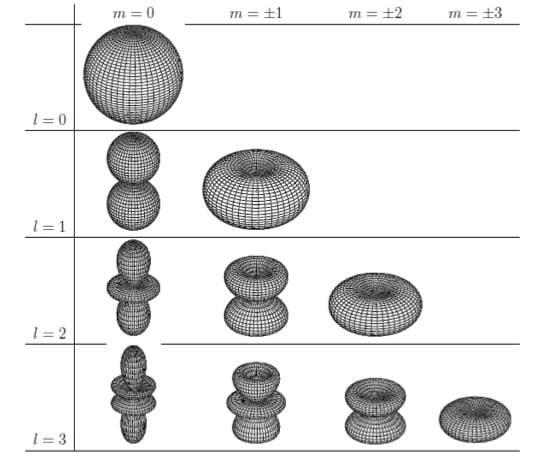
\includegraphics[width=0.7\textwidth]{bilder/schwingungsmoden.jpg}
    \caption{Betrag der Schwingungsmoden $|Y_l^m(\theta{,}\varphi|$. \cite{No}}
\end{figure}

\subsubsection*{Symmetriebrechung}
Ist die Kugelsymmetrie aufgehoben, so wird die Entartung der einzelnen m-Zustände aufgehoben, sodass die verschiedenen Kugelflächenfunktionen
zu einem $l$ nicht mehr die gleichen Energien haben. Da es zu jedem $l$ insgesamt $2l+1$ verschiedene $m$ gibt, sollte 
sich dies im Spektrum äußern. Allerdings wird im Spektrum lediglich eine Gruppe von $l+1$ Peaks deutlich, da sich die weiteren
Zustände nur in der Phase unterscheiden. Bei geringer Verformung können die Kugelflächenfunktionen näherungsweise weiterhin als Lösung angenommen werden.\\
\newline
\subsection{Analogon Wasserstoffatom}
Das Analogon zum Kugelresonator bildet das Wasserstoffatom mit einem einzigen Elektron, was ein analytisches
Lösen der Schrödingergleichung ermöglicht.
Es folgt hierfür die dreidimensionale, zeitunabhängige Schrödingergleichung
\begin{equation}
    E\psi(\vec{r})=-\frac{\hbar^2}{2m}\Delta\psi(\vec{r})+V(r)\psi(r)
\end{equation}
mit dem Coulombpotenzial $V(r)$ des Kerns. Drückt man nun die Gleichung in Kugelkoordinaten aus, 
so folgt durch einen Separationsansatz 
\begin{equation}
    \psi(r{,}\theta{,}\varphi)=Y_l^m(\theta{,}\varphi)R_{n{,}l}(r)
\end{equation}
als Lösung für die Differentialgleichung. Dabei lösen die Kugelflächenfunktionen $Y_l^m$
die rein vom Winkel abhängigen Differentialgleichungen und $R_{n{,}l}(r)$ den Radialteil. Dabei beschreibt
$n$ die Hautquantenzahl. In diesem Index unterscheidet sich das Wasserstoffatom zum Kugelresonator. Das führt dazu, dass die
die Resonanzen der beiden Systeme nicht in der gleichen Reihenfolge im Spektrum auftreten und $l$ ist dabei zu einem bestimmten
$n$ beim Kugelresonator nicht entartet, beim Wasserstoffatom jedoch schon. Grund dafür sind die verschiedenen Potenziale.

\subsection{Gekoppelte Kugelresonatoren}
Mit zwei gekoppelten Kugelresonatoren und einer Blende kann ein Wasserstoffmolekül $\text{H}_2^+$ mit einem Elektron simuliert werden.
Durch verschiedene Blenden kann eine unterschiedlich starke Kopplung dargestellt werden.
Genauso wie beim Rohrresonator mit einer Blende, bildet ich auch beim gekoppelten Kugelresonator mit Blende eine zweite Resonanz aus.
Dies lässt sich auf das Überlappen der einzelnen Atomorbitale zurückführen, die somit ein neues Molekülorbital bilden. Die Überlappung kann auf zwei Arten geschehen.
Dabei können die Vorzeichen jeweils gleich sein (Phasenverschiebung von $0°$) oder unterschiedlich (Phasenverschiebung um $180°$). Man spricht von
bindender oder antibindender Überlappung.\\

\begin{figure}
    \center
    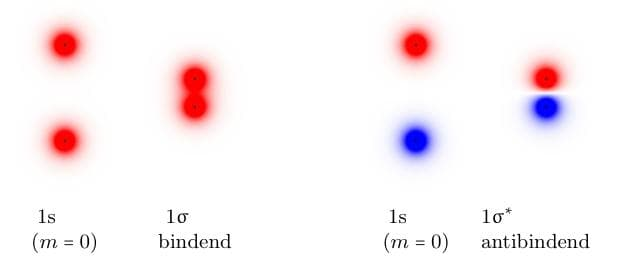
\includegraphics[width=0.7\textwidth]{bilder/mol_orbitale.jpg}
    \caption{Beispiel für bindende und antibindende Molekülorbitale beim Zusammenführen zweier Atome.
    Die Farbe spiegelt dabei die Phase wider. \cite{uni}}
\end{figure}
Zwei Atome mit 1s-Orbitalen bilden somit bei positivem Vorzeichnen ein zugehöriges 1$\sigma$-Molekülorbital. Die neun Orbitale werden dabei mit
griechischen Buchstaben gekennzeichnet und resultieren aus der magnetischen Quantenzahl $m$. Aus $m=0$ folgt somit die neue Orbitalbezeichnung 
$\sigma$, $m=1$ fürt zu einen $\pi$-Orbital.
Die Hautquantenzahl unterscheidet dabei die Orbitale gleicher Symmetrien aber unterschiedlichen Energien.
Zusatzlich kann die Wahrscheinlichkeit der Lage des Elektrons beschrieben werden. Dabei hat das 1$\sigma$ Molekülorbital eine hohe Wahrscheinlichkeit für die Lage zwischen
den beiden Atomkernen (bindender Zustand, energetische tiefere Lage). Bei niedriger Auftrittswahrscheinlichkeit beim
antibinden Zustand 1$\sigma^*$ liegt der Zustand energetisch höher als der Zustand des Atoms.










\section{Durchführung}
\label{sec:Durchfuehrung}
\subsection{Justierung der Apparatur}
Zunächst wird der Aufbau komplett justiert damit die zwei Strahlen nach dem zweiten Glan Thompson Prisma auf die beiden Photowiederstände treffen.
Zur Justierung wird zunächst die Probe und der Interferenzfilter entfernt um den richtigen Strahlengang durch die Magnete und die Probe zu gewährleisten.
\subsection{Winkelmessungen}
\subsection{Magnetfeldmessung}
Mithilfe einer Hall Sonde wird das Magnetfeld innerhalb der Spulen gemessen.
\section{Auswertung}
\subsection{Rohrresonator}
Zunächst wird das Frequenzspektrum von einem bis zwölf aneinander gereihten Zylindern der jeweiligen Länge $50\,$mm
in einem Frequenzbereich von $0,1\,$kHz bis $12\,$kHz mit einem 2-Kanal-Oszilloskop aufgenommen.
Diese Messung wird mit der Software des Computers wiederholt.
Exemplarisch werden im Folgenden die beiden Messungen mit einem, fünf und zwölf Zylindern dargestellt.
Es wird deutlich, dass beide Frequenzspektren ähnlich aussehen. Allerdings ist die Auflösung 
des Spektrums, welches von der Computersoftware aufgezeichnet wurde höher. Es ist daher sinnvoll im Folgenden
diese zu verwenden.

\begin{figure}[H]

    \centering
    \subfloat[Das Frequenzspektrum eines einzelnen Rohrresonators der Länge $50\,$mm (Computersoftware).]{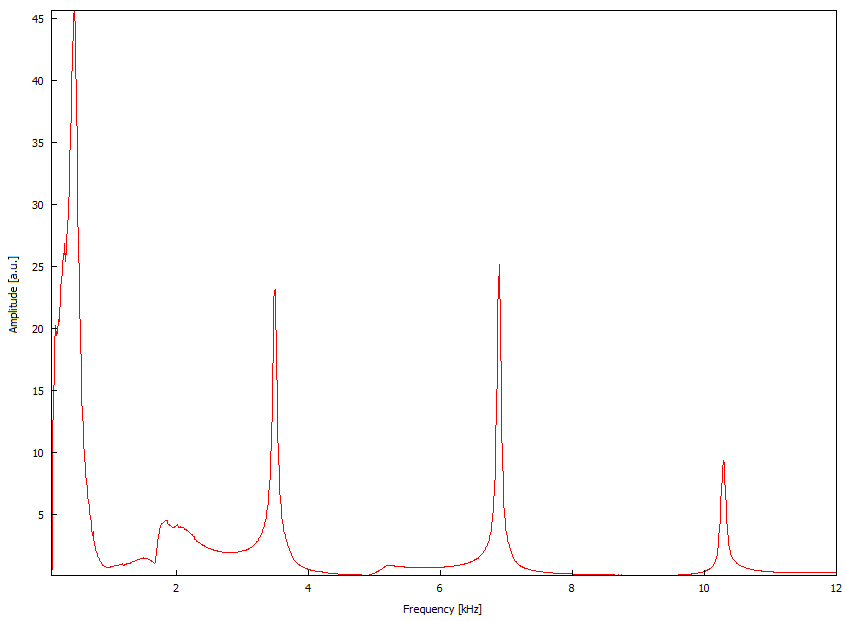
\includegraphics[width=0.45\textwidth]{data/Vorbereitung/Spektrum_1.png}}\hfil
    \subfloat[Das Frequenzspektrum eines einzelnen Rohrrensonators der Länge $50\,$mm (per Oszilloskop).]{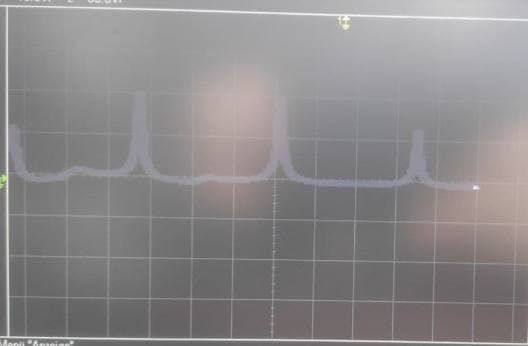
\includegraphics[width=0.45\textwidth]{data/Vorbereitung/Spektrum_1_bild.png}}\hfil 
    
    \subfloat[Das Frequenzspektrum von vier Rohrresonatoren der jeweiligen Länge $50\,$mm (Computersoftware).]{\includegraphics[width=0.45\textwidth]{data/Vorbereitung/Spektrum_4.png}}\hfil
    \subfloat[Das Frequenzspektrum von vier Rohrrensonatoren der jeweiligen Länge $50\,$mm (per Oszilloskop).]{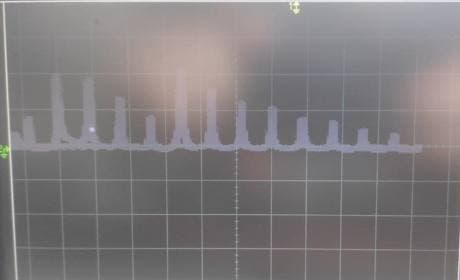
\includegraphics[width=0.45\textwidth]{data/Vorbereitung/Spektrum_4_bild.png}}\hfil

    \subfloat[Das Frequenzspektrum von acht Rohrresonatoren der jeweiligen Länge $50\,$mm (Computersoftware).]{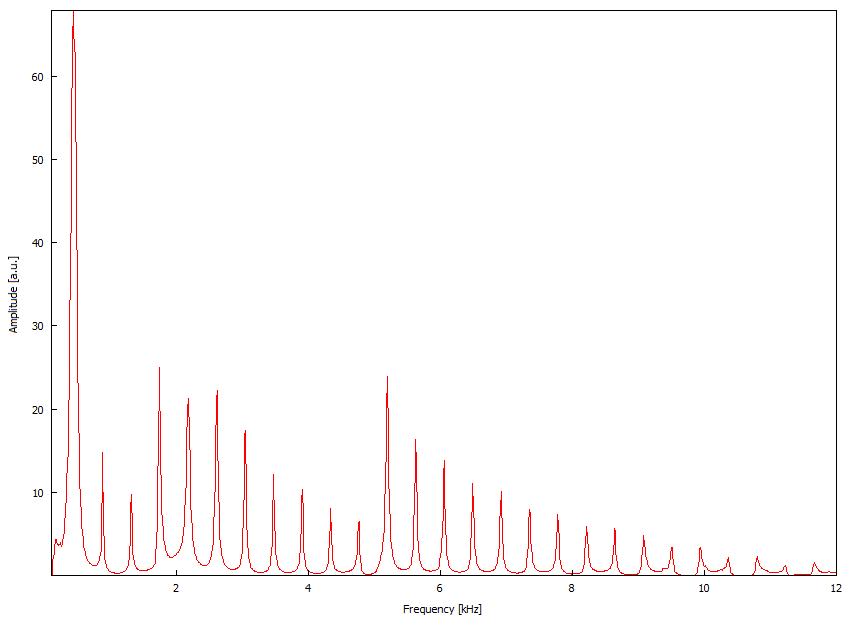
\includegraphics[width=0.45\textwidth]{data/Vorbereitung/Spektrum_8.png}}\hfil
    \subfloat[Das Frequenzspektrum von acht Rohrrensonatoren der jeweiligen Länge $50\,$mm (per Oszilloskop).]{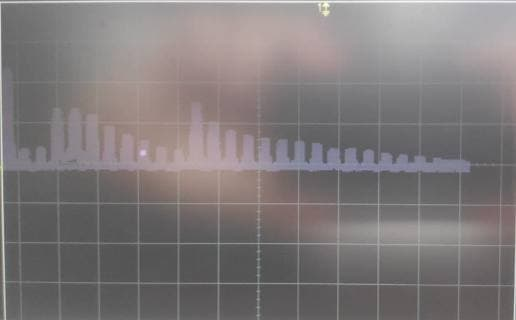
\includegraphics[width=0.45\textwidth]{data/Vorbereitung/Spektrum_8_bild.png}}
    \caption{}\label{figure}
\end{figure}

\subsection{Wasserstoffatom}
Nun wird der Kugelresonator (Wasserstoffatom) betrachtet. Hierbei wird ein Frequenzspektrum
von $0,1\,$kHz bis $12\,$kHz in $5\,$Hz-Schritten aufgenommen. Der Winkel zwischen Mikrofon und Lautsprecher betraägt $180°$.
Die gefunden Resonanzfrequenzen werden anschließend erneut händisch mit dem Sinusgenerator über das Oszilloskop vermessen.
Dies beinhaltet die Ordnung der Resonanz, die Amplitude sowie die Phasenverschiebung neben der Resonanzfrequenz.
Für die Resonanzfrequenzen $X\,$kHz, $Y\,$kHz, $Z\,$kHz und $W\,$kHz wird die Winkelabhängigkeit im Bereich $0°$ bis $180°$ in $10°$-Schritten betrachtet.\\
Zur Analyse der Aufspaltung wird ein Frequenzspektrum in $1$Hz-Schritten im Bereich $1,8$ und $2,8$kHz mit eingesetzten
verschiedener Blenden aufgenommen. Die Abhängigkeit der Resonanzfrequenz vom Winkel wird bei eingesetzter $9$mm Blende 
im Winkelbereich $0\,°$ bis $180\,°$ betrachtet.

\subsubsection*{Resonanzfrequenz}
Im Frequenzbereich zwischen $0,1$ und $12\,$kHz ergibt sich bei einem Winkel von $180\,°$ das in Abbildung \ref{fig:kugel_res}
dargestellte Frequenzspektrum.

\begin{figure}
    \center
    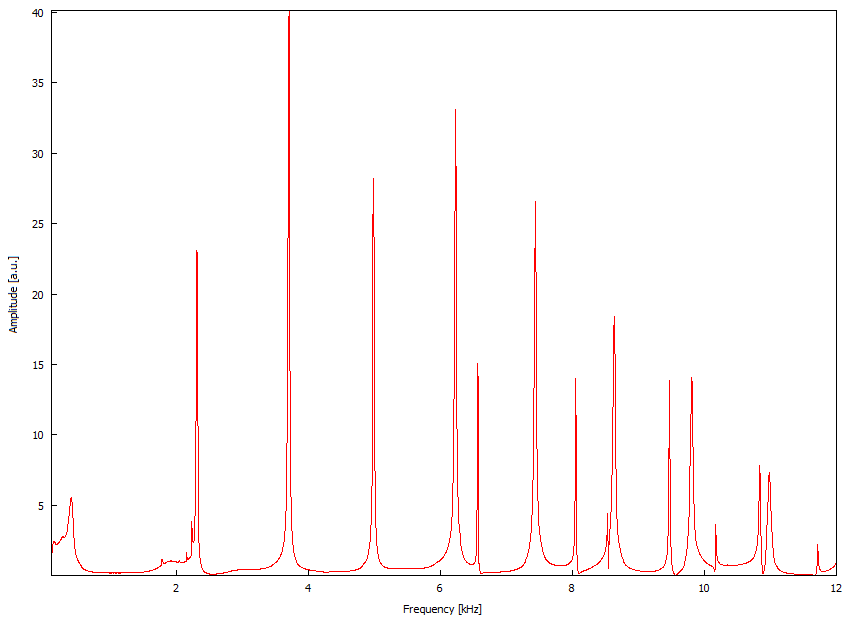
\includegraphics[width=0.7\textwidth]{data/Wasserstoffatom/Ohne_Ring/Spektrum_180_first.png}%{bilder/plots/kugel_180_plot.pdf}
    \caption{Das Hochauflösende Spektrum des Kugelresonators (Wasserstoffatommodells), bei einem 
    festen Polarwinkel von $180°$. Dabei ist die Frequenz in kHz gegen die Amplitude in willkürlichen Einheiten aufgetragen.}
    \label{fig:kugel_res}
\end{figure}

Die genauere Betrachtung der Resonanzfrequenzen $\nu_{res}$ aus Abbildung \ref{fig:kugel_res} mithilfe des Oszilloskops
liefert die jeweilige Ordnung, Amplitude und Phasenverschiebung.

\begin{table}[H]
    \center
    \caption{Die zu den Resonanzfrequenten $\nu_{Res}$ gehörigen Ordnungen, Amplituden und Phasenverschiebungen.}
    \begin{tabular}{l l l c}
        \toprule
        Ordnung & $\nu_{Res}\,/\,$kHz & Amplitude$\,/\,$V & $\varphi\,/\,°$\\
        \midrule
        1 &0,4   &4,3  & -102  \\
        2 &2,301 &76   &   70  \\
        3 &3,694 &231  &  -78  \\
        4 &4,979 &187  &   90  \\
        5 &6,221 &249  &  -30  \\
        6 &7,433 &239  &  170  \\
        7 &8,042 &143  &  -14  \\
        8 &8,630 &189  &   20  \\
        9 &9,465 &155  & -150  \\
        10&9,807 &159  & -130  \\
        \bottomrule
    \end{tabular}
\end{table}


\subsubsection{Die Winkelabhängigkeit der Resonanzfrequenzen}
Nun wird die Druckamplitude der Resonanzfrequenzen $2,301\,$kHz, $3,694\,$kHz, $4,979\,$kHz und $7,433\,$kHz 
in Abhängigkeit des Winkels $\theta$ betrachtet.\\
Deutlich zu ernennen sind die Keulen in $180°$-Richtung, sowie eine schwache Ausprägung in $90°$-Richtung.

\begin{figure}[H]
    \centering
    \subfloat[Die Druckamplitude bei der Resonanzstelle $2,300$kHz (Form eines $2{p}_0$-Orbitals).]{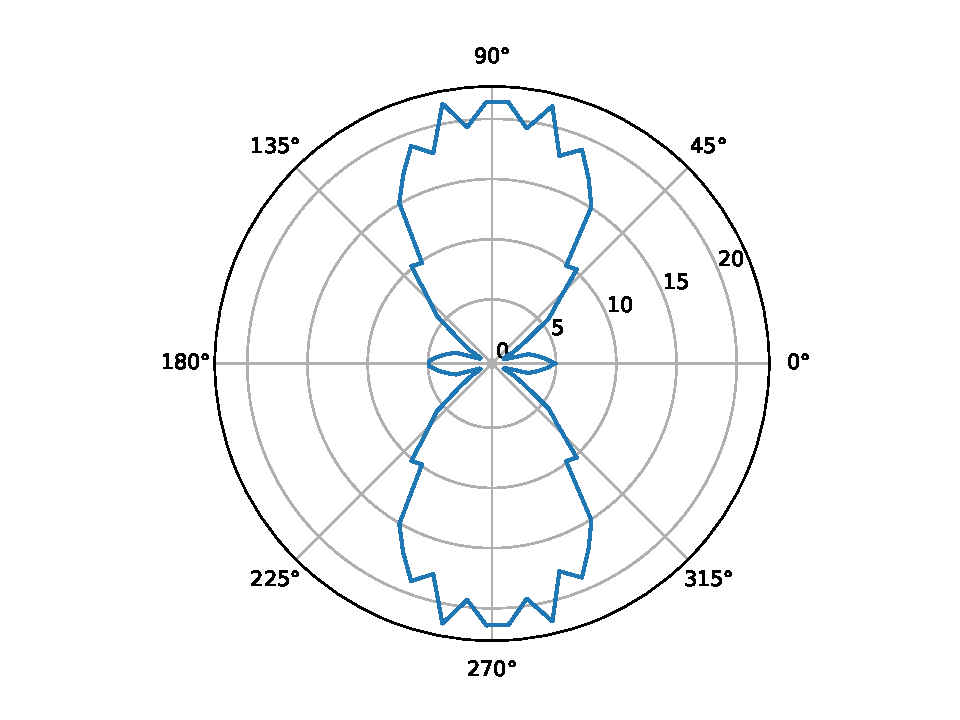
\includegraphics[width=0.45\textwidth]{plots/Hatom/polar_2300.pdf}}\hfil
    \subfloat[Die Druckamplitude bei der Resonanzstelle $3,690$kHz (Form eines $3{d}_0$-Orbital).]{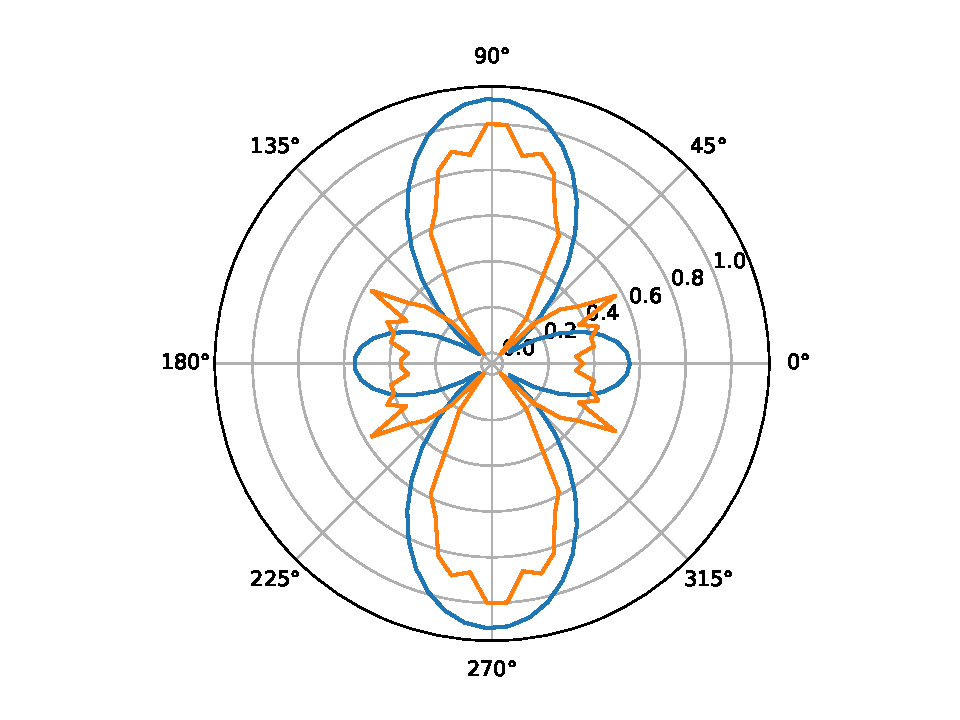
\includegraphics[width=0.45\textwidth]{plots/Hatom/polar_3960.pdf}}\hfil 
    
    \subfloat[Die Druckamplitude bei der Resonanzstelle $4,970$kHz (Form eines $4{f}_0$-Orbital).]{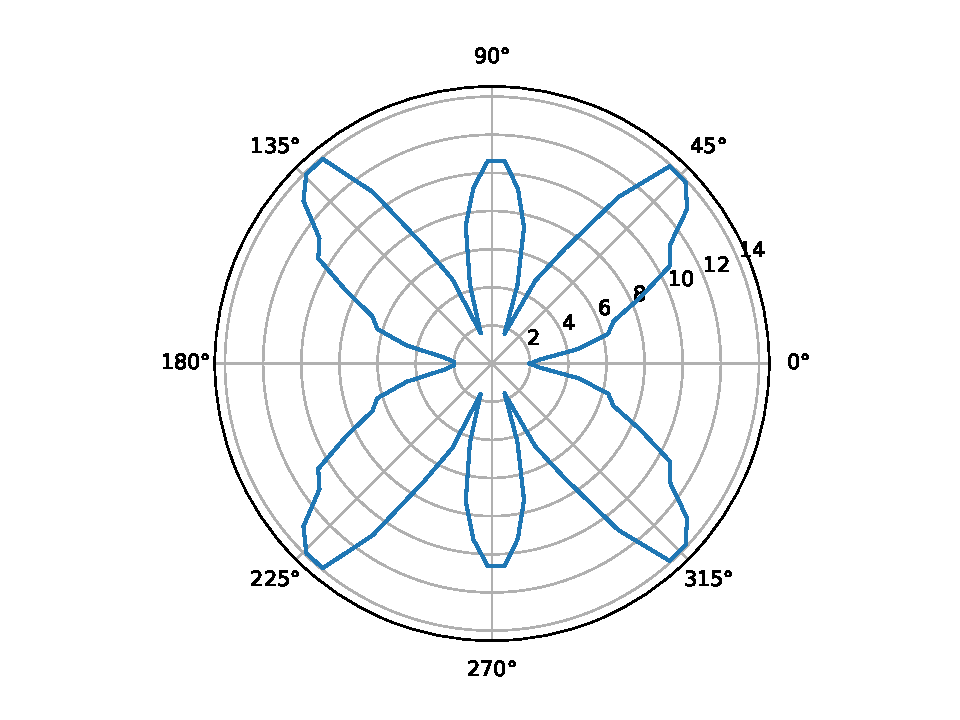
\includegraphics[width=0.45\textwidth]{plots/Hatom/polar_4970.pdf}}\hfil
    \subfloat[Die Druckamplitude bei der Resonanzstelle $7,430$kHz (Form eines $6{h}_0$-Orbital).]{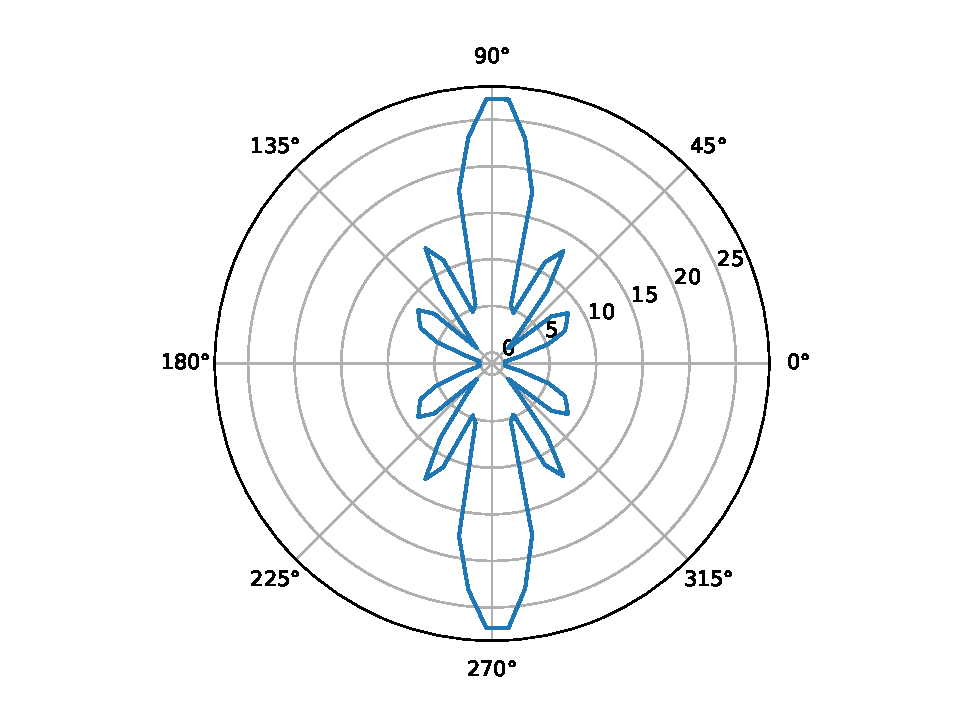
\includegraphics[width=0.45\textwidth]{plots/Hatom/polar_7430.pdf}}\hfil 
    \caption{}\label{figure}
\end{figure}
\subsubsection*{Aufspaltung der Zustände}
Nun werden verschiedene Zwischenringe zwischen den beiden Halbkugel eingesetzt. Exemplarische wird im folgenden das Zwischenstück
mit einer Ringbreite von $3$mm betrachtet. In Abbildung \ref{fig:aufspaltung} sind die zwei resultierenden Resonanzfrequenzen
deutlich. Die Drehimpulsquantenzahl $l$ muss daher gleich eins sein und bestätigt die Annahme, dass es sich um ein 2p$_0$-orbital handelt.  

\begin{figure}[H]
    \center
    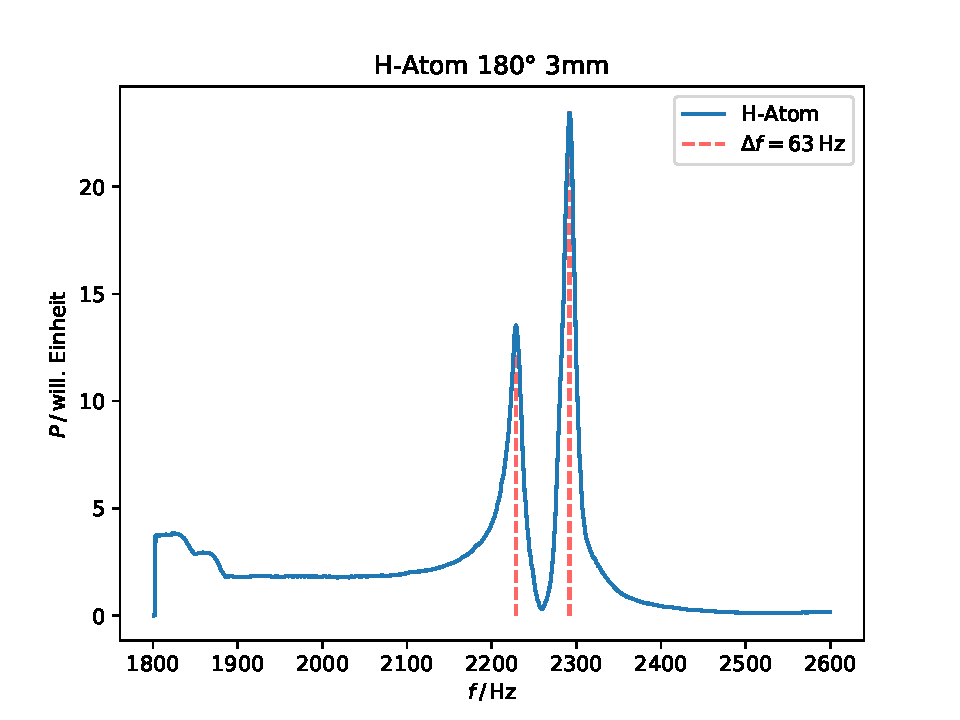
\includegraphics[width=0.8\textwidth]{plots/Hatom/zustandsaufspaltung.pdf}
    \caption{Aufspaltung der Resonanz bei $2,301$kHz in zwei Resonanzfrequenzen.}
    \label{fig:aufspaltung}
\end{figure}

Trägt man nun die die Resonanzfrequenz-Differenz $\Delta\nu$ gegen die Zwischenringbreite auf,
so wird deutlich, dass sich dies annähernd linear verhält (vgl. Abblindung \ref{fig:d_res}). Analogon hierfür wäre die Aufspaltung der Zustände eines
Wasserstoffatoms in einem extern anliegendem Magnetfeld (Zeeman-Effekt).

\begin{figure}[H]
    \center
    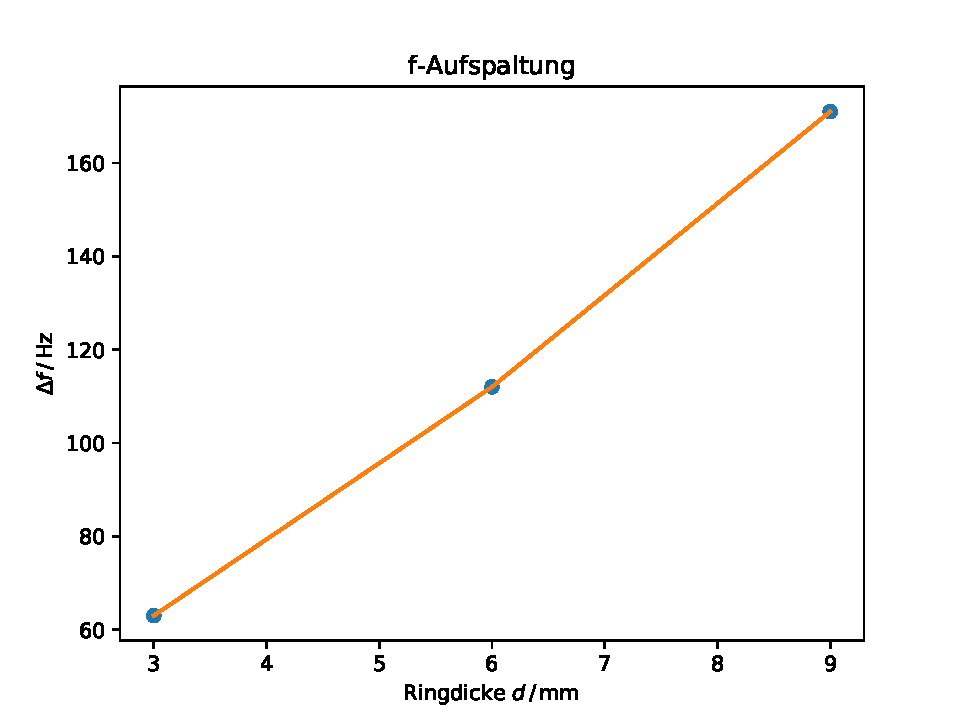
\includegraphics[width=0.8\textwidth]{plots/Hatom/faufspaltung.pdf}
    \caption{Abhängigkeit zwischen der Resonanzfrequenz-Differenz $\Delta\nu$ und der Ringbreite.}
    \label{fig:d_res}
\end{figure}
\newpage
\subsubsection*{Zustandsaufspaltung und deren Winkelabhängigkeit}
%Für einen Zwischenring der Ringbreite $9$mm wird im Folgenden die Winkelabhängigkeit betrachtet (Abbildung \ref{fig:9mm_winkel}).

%\begin{figure}[H]
%    \center
%    \includegraphics[width=0.5\textwidth]{example-image-a}
%    \caption{Druckamplitude gegen den Winke $\theta$ aufgetragen.}
%    \label{fig:9mm_winkel}
%\end{figure}

Für die Aufspaltung bei $180°$ ergibt sich das Frequenzspektrum aus Abbildung \ref{fig:9mm_res}.
Die Resonanzfrequenz $2,095$kHz entspricht $m=0$ und $l=1$. Für die Resonanzfrequenz $2,265$kHz folgt $m=\pm 1$ und $l=1$.
\begin{figure}[H]
    \center
    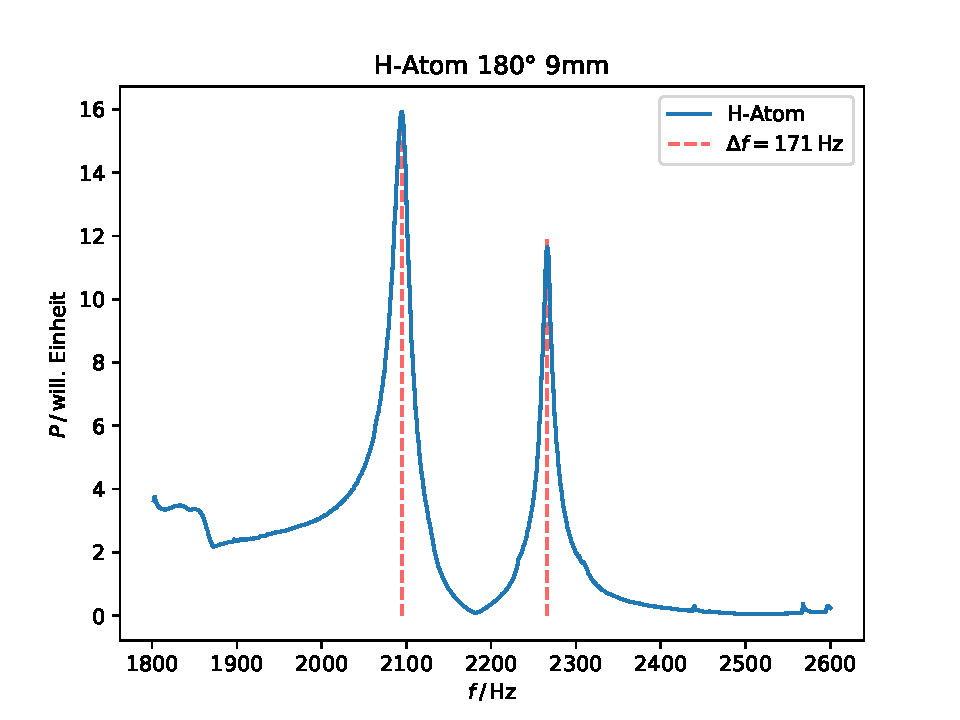
\includegraphics[width=0.7\textwidth]{plots/Hatom/zustandsaufspaltung_9.pdf}
    \caption{Die Aufspaltung der Resonanz bei Verwendung eines Zwischenrings der Breite $9$mm bei einem Winkel $\theta$ von $180°$.}
    \label{fig:9mm_res}
\end{figure}
\newpage
\subsection{Wasserstoffmolekül}
\subsubsection*{Einfluss des Blendendurchmessers auf die Resonanzfrequenz}
Nun werden zwei Kugelresonatoren über eine Blende, welche die Kopplungsstärke wiederspiegelt, gekoppelt.
Zur Untersuchung wird zunächst ein Frequenzspektrum im Bereich von $2,2\,$kHz bis $2,5\,m$kHz in $1\,$Hz-Schritten bei verschiedenen
Blenden von $10\,$mm, $16\,$mm, $20\,$mm betrachtet.\\

Für das Resonanzfrequenz $f$ in Abhängigkeit des Blendendurchmessers zeigt sich folgender in Abbildung \ref{fig:blende_mol}
Verlauf.
\begin{figure}[H]
    \center
    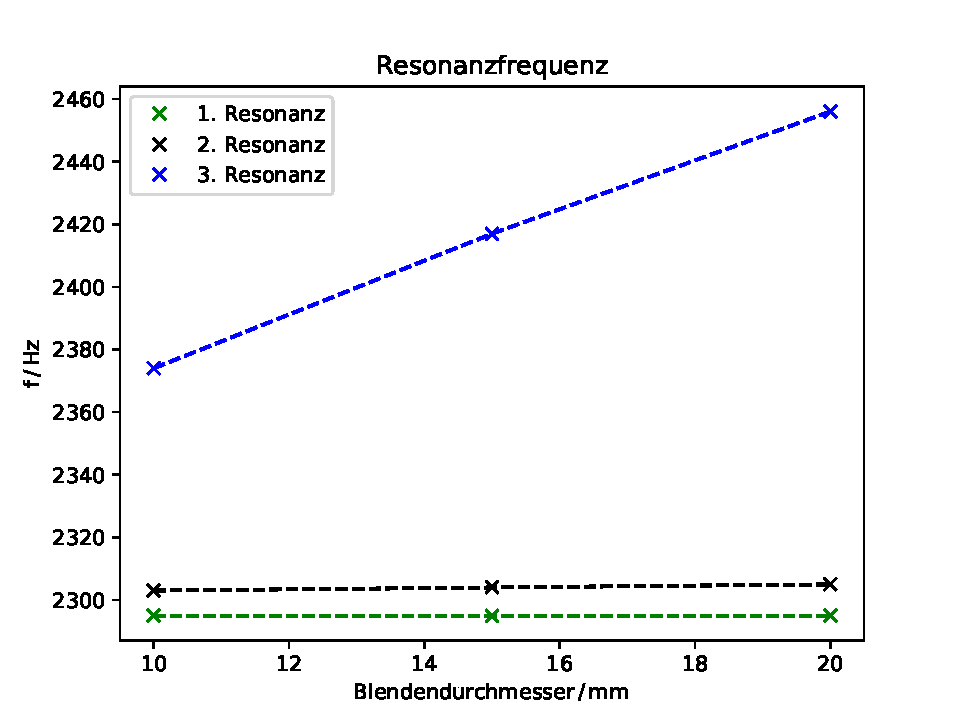
\includegraphics[width=0.7\textwidth]{plots/Hatom/res_blende.pdf}
    \caption{Abhängigkeit der 3 Resonanzfrequenzen zum Blendendurchmesser.}
    \label{fig:blende_mol}
\end{figure}

\subsubsection*{Winkelabhängigkeit der Resonanzfrequenz}
Für den Blendendurchmesser von $15$mm zeigen sich die drei Resonanzen, dargestellt in Abbildung \ref{fig:blende_16_res},
bei den Frequenzen $\nu$ von $2,297$kHz, $2,304$kHz und $2,416$kHz.
\begin{figure}[H]
    \center
    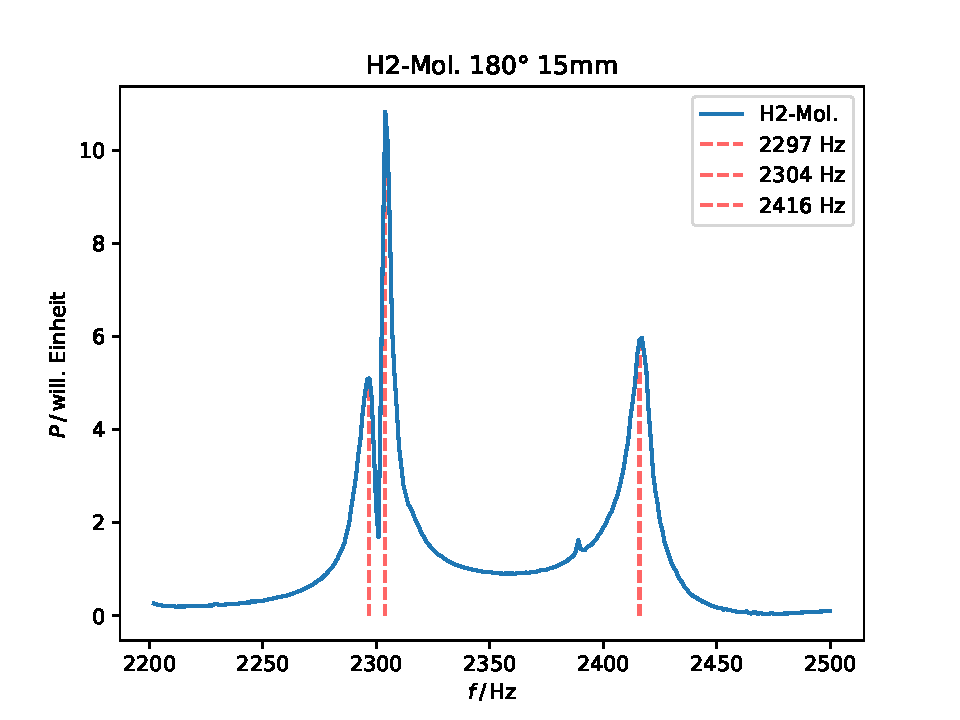
\includegraphics[width=0.7\textwidth]{plots/Hatom/zustandsaufspaltung_mol15.pdf}
    \caption{Frequenzspektrum bei einem Winkel $\theta=180°$. Zu sehen sind die Resonanzenfrequenzen $\nu$ bei $2,297$kHz, $2,304$kHz und $2,416$kHz.}
    \label{fig:blende_16_res}
\end{figure}

Im Folgenden werden für diese vier Resonanzfrequenzen die Druckamplituden in Abhängigkeit des Winkels $\theta$ betrachtet und die Phasenverschiebung in Tabelle \ref{tab:mol_diff} aufgelistet.
Daraus lassen sich die Symmetrien der Zustände definieren. Für eine Phasendifferenz von $0°$ spricht man von einem symmetrischen und bei einer Phase von $180°$ von einem antisymmetrischen Zustand.
%VERGLEICHE LASSE
\begin{figure}[H]
    \centering
    \subfloat[Die Druckamplitude bei der Resonanzstelle $2,297$kHz]{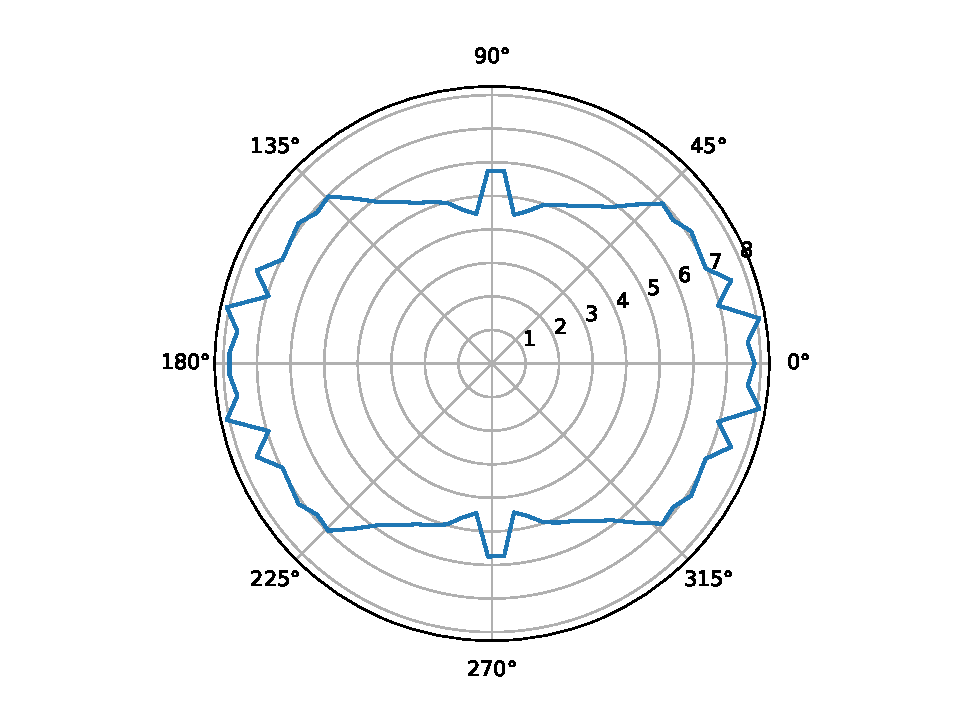
\includegraphics[width=0.45\textwidth]{plots/Hatom/polar_mol_2297.pdf}}\hfil
    \subfloat[Die Druckamplitude bei der Resonanzstelle $2,304$kHz ]{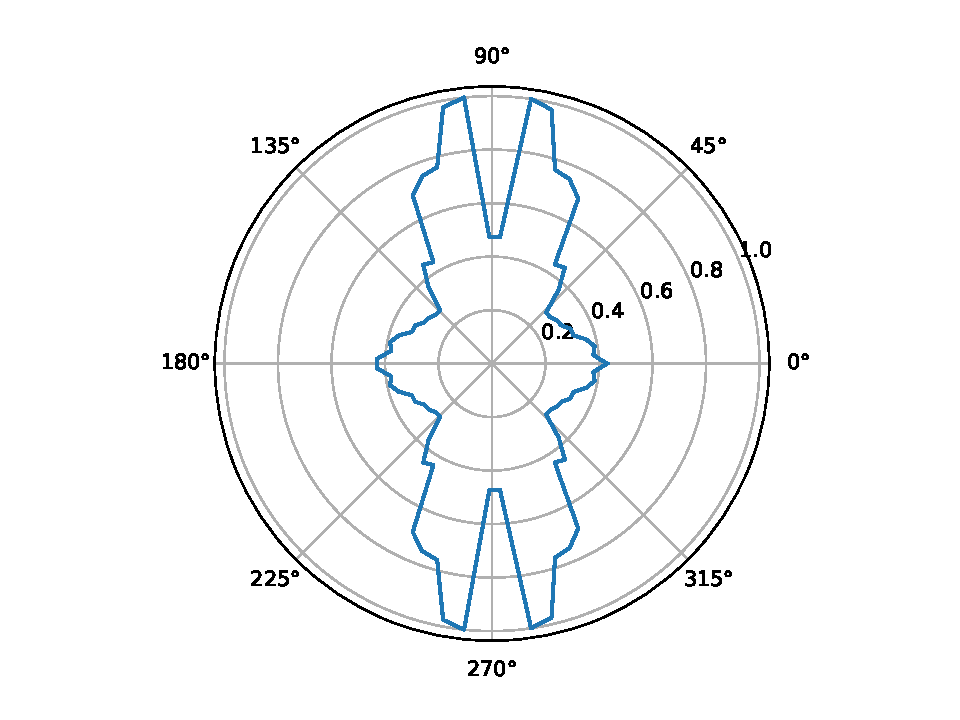
\includegraphics[width=0.45\textwidth]{plots/Hatom/polar_mol_2304.pdf}}\hfil 
    
    \subfloat[Die Druckamplitude bei der Resonanzstelle $2,416$kHz ]{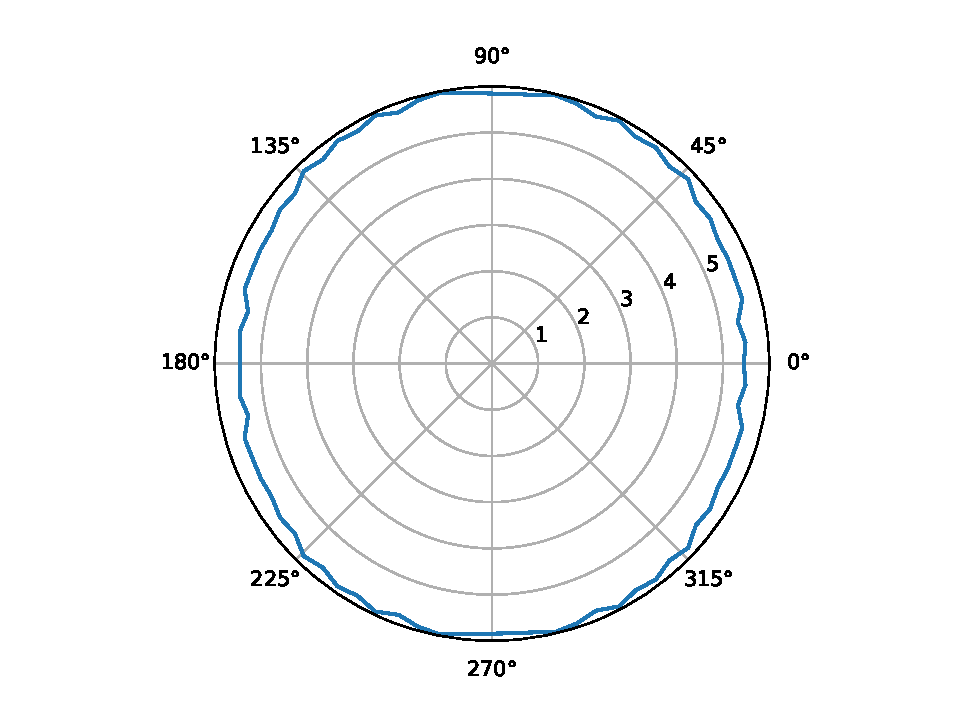
\includegraphics[width=0.45\textwidth]{plots/Hatom/polar_mol_2416.pdf}}\hfil
    \caption{}
    \label{fig:polarplots}
\end{figure}

\begin{table}
    \center
    \caption{}
    \begin{tabular}{c| c c c c}
        \toprule
        Ordnung & $\nu_{Res}\,/\,$kHz & obere Phasendiff. $\,/\,°$ & untere Phasendiff. $\,/\,°$ & $\Delta$ Phasendiff. $\,/\,°$\\
        \midrule
        1 &2,296 &-135 &10 &145 \\
        2 &2,303 &-126 &30 &156 \\
        3 &2,418 &53 &-128 &181 \\
        \bottomrule
    \end{tabular}
    \label{tab:mol_diff}
\end{table}
\newpage
\subsection{1-dim-Festkörper}
\subsubsection*{Resonatorkette}
Nun wird ein Frequenzspektrum einer Resonatorkette betrachtet die mit jeweils $16$mm-Blenden versehen werden.
In Abbildung \ref{fig:reskette_res} prägen sich vier Bereiche aus, die mit Maxima gefüllt sind. Dabei entspricht dies der Anzahl der Maxima der verwendeten Zylinder.
Überträgt man dies auf das Analogon des 1-dim-Festkörpers so lässt sich sagen, dass durch jeden Zylinder ein Band hinzugeführt wird, auf dem die Elektronen
in eine Festkörper Zustände einnehmen können. Die leeren Bereiche sind dabei Bandlücken und beschreiben somit die 'verbotenden' Zonen im Festkörper in denen keine Elektronenzustände vorliegen.


\begin{figure}[H]
    \centering
    \subfloat[Frequenzspektrum für eine Resonatorkette aus zwei Resonatorgliedern (Rohrzylindern) mit einer jeweiligen Länge von $50$mm und einer $16$mm-Blende als Zwischenstück.]{\includegraphics[width=0.45\textwidth]{data/Festkoerper/16mm/Spektrum_2.png}}\hfil
    \subfloat[Frequenzspektrum für eine Resonatorkette aus vier Resonatorgliedern (Rohrzylindern) mit einer jeweiligen Länge von $50$mm und einer $16$mm-Blende als Zwischenstück.]{\includegraphics[width=0.45\textwidth]{data/Festkoerper/16mm/Spektrum_4.png}}\hfil 
    
    \subfloat[Frequenzspektrum für eine Resonatorkette aus zehn Resonatorgliedern (Rohrzylindern) mit einer jeweiligen Länge von $50$mm und einer $16$mm-Blende als Zwischenstück..]{\includegraphics[width=0.45\textwidth]{data/Festkoerper/16mm/Spektrum_10.png}}\hfil
    \caption{}
    \label{fig:reskette_res}
\end{figure}

\subsubsection{Resonatorkette mit verschiedenen Blendendurchmessern}
Die Größe des Blendendurchmessers spiegelt im Analogon des 1-dim-Festkörpers ein unterschiedlich starkes
Potenzial wieder, sodass die Elektronen unterschiedlich stark lokalisiert auf ihren Bändern sind.
Dies wird deutlich, wenn man sich das Frequenzspektrum zweier Resonatorketten mit unterschiedlichen Blenden betrachtet.
Dazu ist in Abbildung \ref{fig:fest_2_blende} jeweils das Frequenzspektrum einer Resonatorkette mit zwei Zylindern und einer $10$mm-Blende
und gleiche Resonatorkette mit einer $13$mm-Blende dargestellt.\\
\begin{figure}[H]
    \centering
    \subfloat[Frequenzspektrum einer Resonatorkette bestehend aus zwei Rohrzylindern der Länge 50mm und eine Blende mit dem Durchmesser von 10mm.]{\includegraphics[width=0.45\textwidth]{data/Festkoerper/10mm/Spektrum_2.png}}\hfil
    \subfloat[Frequenzspektrum einer Resonatorkette bestehend aus zwei Rohrzylindern der Länge 50mm und eine Blende mit dem Durchmesser von 13mm.]{\includegraphics[width=0.45\textwidth]{data/Festkoerper/13mm/Spektrum_2.png}}\hfil 
    \caption{}
    \label{fig:fest_2_blende}
\end{figure}

\begin{figure}[H]
    \centering
    \subfloat[Frequenzspektrum einer Resonatorkette bestehend aus vier Rohrzylindern der Länge 50mm und eine Blende mit dem Durchmesser von 10mm.]{\includegraphics[width=0.45\textwidth]{data/Festkoerper/10mm/Spektrum_4.png}}\hfil
    \subfloat[Frequenzspektrum einer Resonatorkette bestehend aus vier Rohrzylindern der Länge 50mm und eine Blende mit dem Durchmesser von 13mm.]{\includegraphics[width=0.45\textwidth]{data/Festkoerper/13mm/Spektrum_4.png}}\hfil 
    \caption{}
    \label{fig:fest_4_blende}
\end{figure}

\begin{figure}[H]
    \centering
    \subfloat[Frequenzspektrum einer Resonatorkette bestehend aus zehn Rohrzylindern der Länge 50mm und eine Blende mit dem Durchmesser von 10mm.]{\includegraphics[width=0.45\textwidth]{data/Festkoerper/10mm/Spektrum_10.png}}\hfil
    \subfloat[Frequenzspektrum einer Resonatorkette bestehend aus zehn Rohrzylindern der Länge 50mm und eine Blende mit dem Durchmesser von 13mm.]{\includegraphics[width=0.45\textwidth]{data/Festkoerper/13mm/Spektrum_10.png}}\hfil 
    \caption{}
    \label{fig:fest_10_blende}
\end{figure}
Es wird deutlich, dass die jeweiligen Maxima-Ausschläge deutlich höhere Werte annehmen für den jeweiligen Konfiguartionen mit der größeren Blende.


\subsubsection*{Störstellen im Festkörper}
Durch Verwendung vereinzelt geänderter Zylinderlängen können Störstellen, die im Festkörper Gitterdefekte entsprechen, simuliert werden.
Diese führen zu Abweichungen im Frequenzspektrum, verglichen zum ungestörten Frequenzspektrum.
Konkret lassen sich für die Störzylinder der Größe $37,5\,$mm und $62,5\,$mm eine neue Resonanz erkennen. Des weiteren resultiert eine
deutlich sichtbare Verringerung der gesamten Druckamplitude im Vergleich zur ungestörten Resonatorkette. 

\begin{figure}[H]
    \centering
    \subfloat[Fehlstelle mit $37,5$mm Zylinder.]{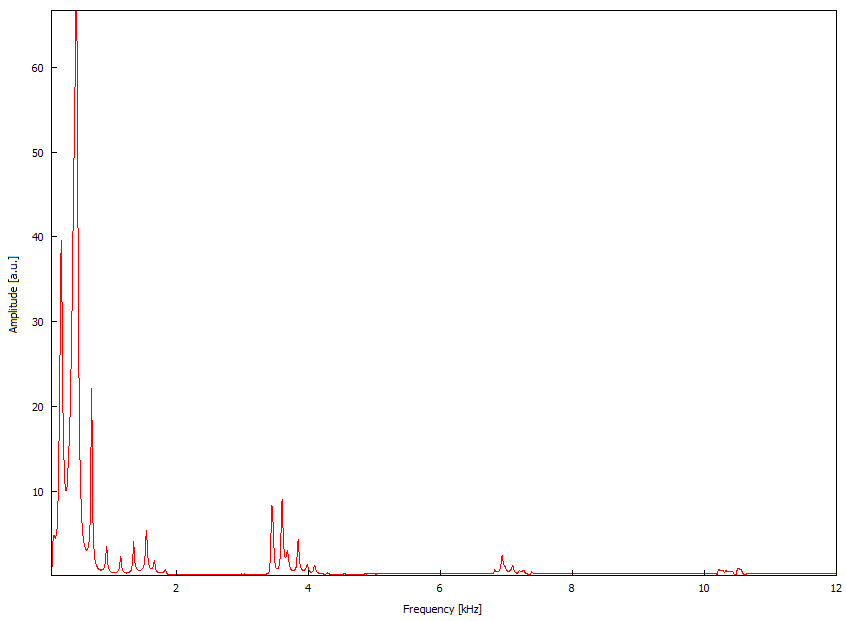
\includegraphics[width=0.45\textwidth]{data/Festkoerper/10mm/Spektrum_dotiert_37_5.png}}\hfil
    \subfloat[Fehlstelle mit $62,5$mm Zylinder.]{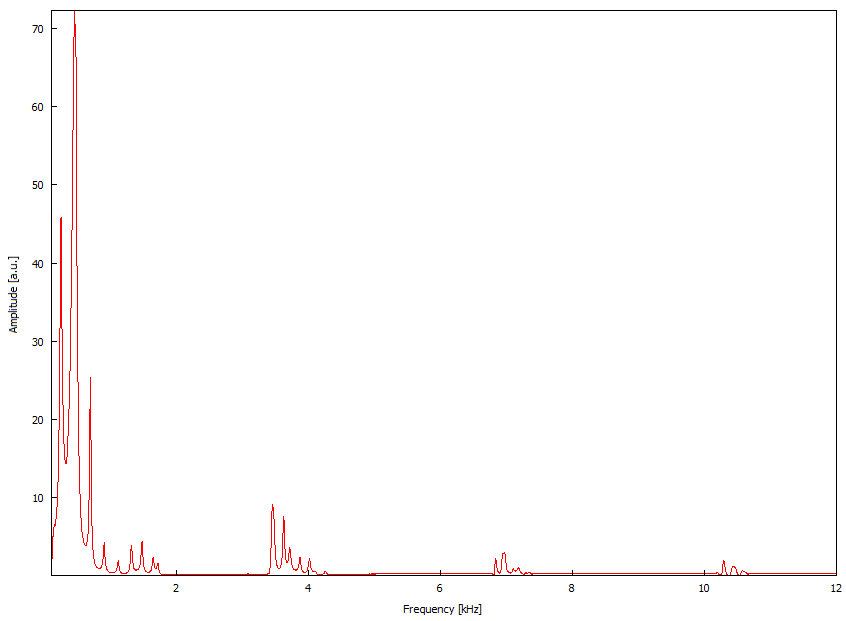
\includegraphics[width=0.45\textwidth]{data/Festkoerper/10mm/Spektrum_dotiert_62_5.png}}\hfil 
    \subfloat[Fehlstelle mit $75$mm Zylinder.]{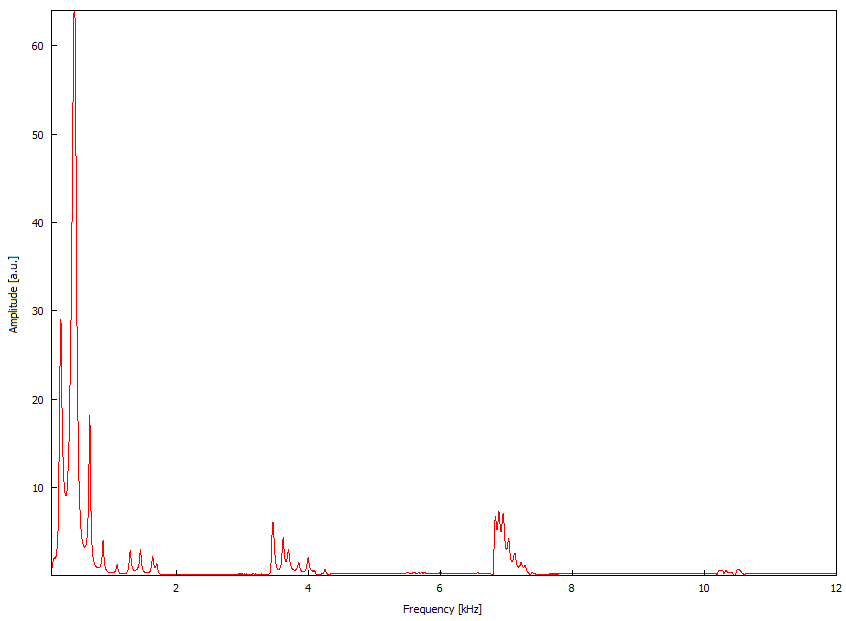
\includegraphics[width=0.45\textwidth]{data/Festkoerper/10mm/Spektrum_dotiert_75.png}} 
    \caption{Frequenzspektren für eine Resonatorkette aus neun Zylindern der Länge $50\,$mm und einer Störstelle durch einen Zylinder einer anderen Länge. Zwischenstücke bilden $10\,$mm Blenden.}
    \label{fig:fest_stoer}
\end{figure}

\subsubsection*{Resonatorkette mit wechselnden Zylinderlängen}
Nun wird eine Resonatorkette aus abwechselnden Zylindern mit den Längen $50\,$mm und $75\,$mm betrachtet.
Dies entspricht einer zwei-atomigen-Festkörper-Basis. Deutlich werden nun, dass die Resonanzen der einzelnen ein-atomigen Basen in 
die zwei-atomigen-basen übernommen werden.\\
In Abbildung \ref{fig:abwech_zylin} wird nun die wechselnde Resonatorkette mit einer $50\,$mm und einer $75\,$mm Resonatorkette verglichen.

\begin{figure}[H]
    \centering
    \subfloat[Frequenzspektrum eines einzelnen Zylinders mit der Länge von $75\,$mm.]{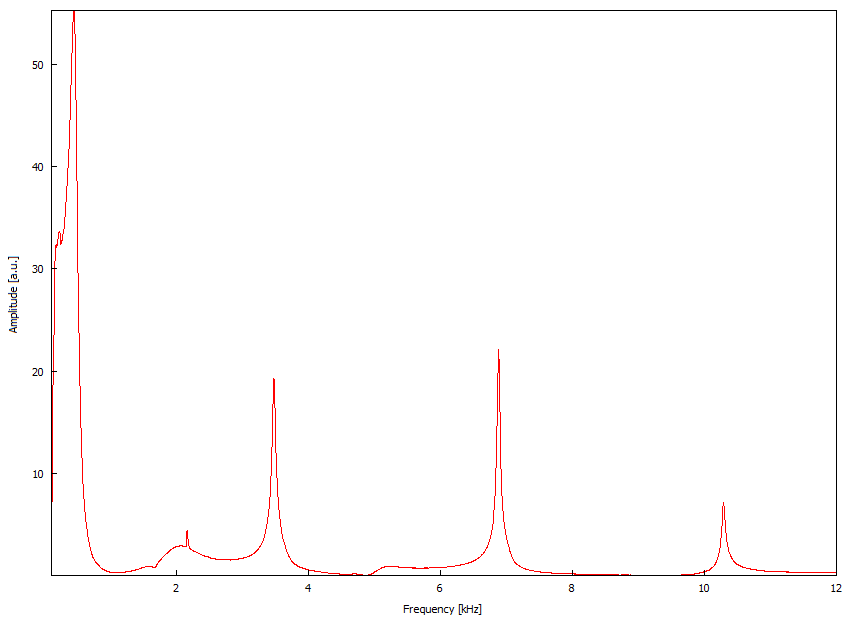
\includegraphics[width=0.5\textwidth]{data/Festkoerper/periodisch/Spektrum_75_einzeln.png}}\hfil
    \subfloat[Frequenzspektrum eines einzelnen Zylinders mit der Länge von $50\,$mm.]{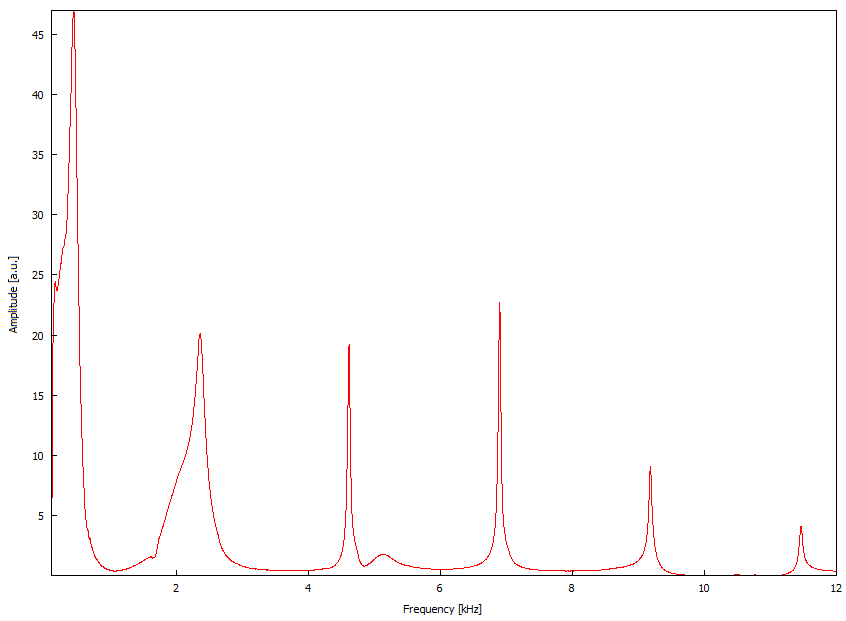
\includegraphics[width=0.5\textwidth]{data/Festkoerper/periodisch/Spektrum_50_einzeln.png}}\hfil 
    \subfloat[Frequenzspektrum einer Resonatorkette mit zehn wechselden Zylindern der Länge $50\,$mm und $75\,$mm und Blenden mit einem Durchmesser von $16\,$mm.]{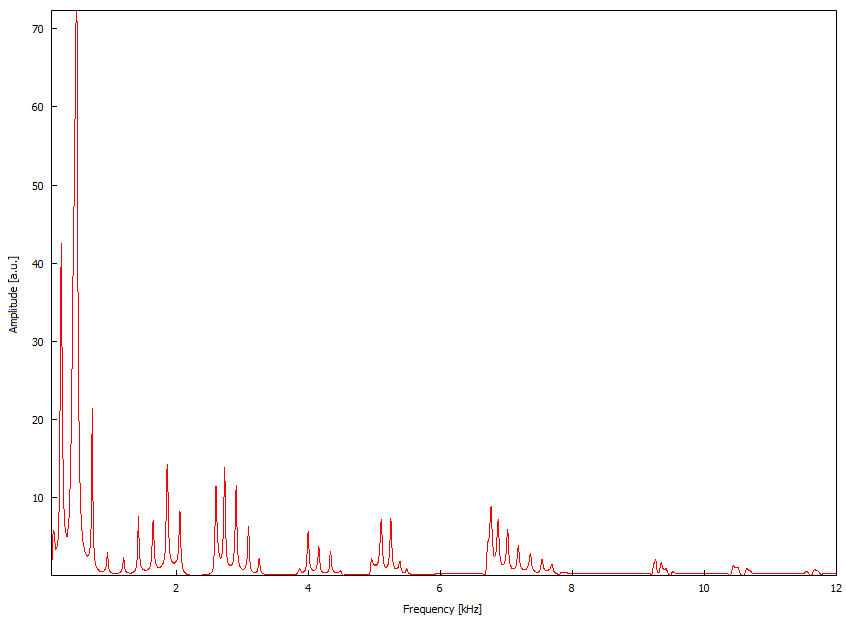
\includegraphics[width=0.8\textwidth]{data/Festkoerper/periodisch/Spektrum_10_16mm_50_75.png}} 
    \caption{}
    \label{fig:abwech_zylin}
\end{figure}

\subsubsection*{Resonatorkette mit wechselndem Blendendurchmesser}
In Abbildung \ref{fig:abwech_blende} ist das Frequenzspektrum einer Resonatorkette aus acht Zylindern mit abwechselden Blendendurchmessern
von $13\,$mm und $16\,$mm dargestellt. Es zeigt sich eine deutliche Aufspaltung der Maximalbereiche.
Auf einen Festkörper übertragen lässt sich somit sagen, dass das vorliegende Gitter nun eine übergeordnete Periodizität aufweist und diese durch
das verschiedene Potenzial entsteht.

\begin{figure}
    \center
    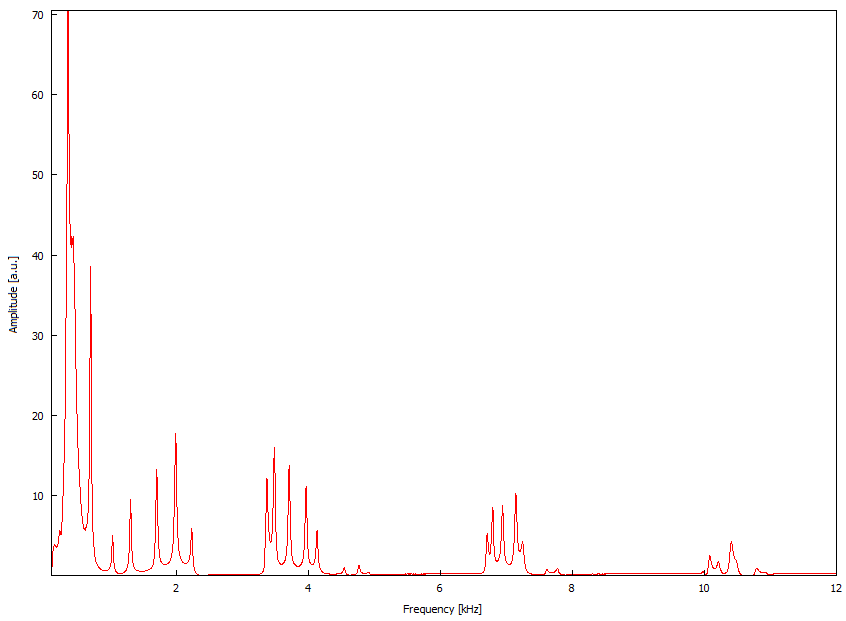
\includegraphics[width=0.8\textwidth]{data/Festkoerper/periodisch/Spektrum_8_13mm_16mm_50.png}
    \caption{Frequenzspektrum einer Resonatorkette aus acht $50\,$mm langen Zylindern, welche abwechselnd durch $13$mm und $16$mm-Blenden getrennt sind.}
    \label{fig:abwech_blende}
\end{figure}

\newpage
\section{Diskussion}
Im dem Versuch wurden die Komponenten eines HeNe-Lasers analysiert. Hierbei wurde zunächst die
Stabilitätsbedingung bei verschiedenen Resonator-Spiegeln-Konfigurationen überprüft. 
Dabei ist deutlich geworden, dass sich für die konkav/konkav Anordnung ($r_1=r_2$) sowie für
die plan/konkav Anordnung eine kritische Stabilität bei einer Resonatorlänge von $1,40\,$m finden lässt.
eine maximale Resonatorlänge konnte sich für die konkav/konkav Anorndung bei $2,80\,$m finden.
Da die Apperatur aufgrund ihrer optischen Schiene auf $2\,$m begrenzt ist, ist diese allerdings von nachrangigier Bedeutung.
Die letzte erfolgreiche Messung konnte dabei bei plan/konkav bis $1,30\,$m durchgeführt werden, da die Justierung mit
steigender Resonatorlänge zunehmend schwieriger wird.\\
Die Messung der verschiedenen Moden deckt sich mit der theoretischen Intensitätsverteilung.
Besonders bei der TEM$_{00}$-Mode folgen die Messungen der vorhergesagten Theoriekurve. Bei der TEM$_{10}$ decken sich Theorie und Messung 
nicht so genau wie bei der TEM$_{10}$-Messung. Dies könnte über weiter Messungen und kleinere Schrittweiten in x-Richtung verbessert werden.
Auch die Reduzierung von Störlicht könnte eine messbare Verbesserung bewirken, da durch die so schon kleinen Interferenzmaxima der TEM$_{10}$-Mode
weiteres Licht die Messung stark beeinflussen.
Allerdings kann man auch hier die Theorie an den Messwerten erkennen.
Die Analyse der Polarisation zeigt wie erwartet eine Periodizität von $\pi$. Die konstante Phase die
durch die Interpolation der Messwerte mit der Theorie ermittelt wurde, folgt dabei aus dem nicht perfekt
parallel ausgerichteten Laser.\\
Bei der Bestimmung der Wellenlänge konnte mithilfe verschiedener Beugungsgitter die Wellenlänge durch eine Mittlung auf
$\bar{\lambda}=651,71\,$nm bestimmt werden. Die theoretische Wellenlänge des Lasers ist mit $\lambda_{\text{Theo}}=632,8\,$nm bekannt.
Somit folgt eine Abweichung von ca. $3\,$\% zum theoretischen Wert und ist somit ein zufriedenstellendes Ergebnis.
Die Abweichung können dabei weiter verkleinert werden, indem weitere Beugungsmaxima weiterer $n$-ter Ordnung für die jeweiligen Beugungsgitter
vermessen werden. Zudem könnte die Ungenauigkeit in der Abstandsmessung durch ein Laser-Abstandsmessgerät stark verringert werden gegenüber der Messung mit Massband und Geodreieck.
\label{sec:Diskussion}
\newpage
\nocite{*}
\printbibliography
\newpage
\section{Anhang}
\label{sec:Anhang}
\begin{figure}[H]
    \centering
    \includegraphics[width = 0.75\textwidth]{./plots/rate_20Hz_plateau.pdf}
    \caption{Versuch eine Plateaufunktion an die Daten zu Fitten. Die Plateaufunktion ist in Formel \ref{eqn:plateau} gezeigt. Die Plateaufunktion ist in diesem Fall eine Potenz der Gaußfunktion.}
    \label{fig:plateau}
\end{figure}
\begin{equation}
    a \cdot e^{-\left(\frac{x-b}{2c}\right)^{64}}
    \label{eqn:plateau}
\end{equation}

\begin{figure}[H]
    \centering
    \includegraphics[width = 0.75\textwidth]{./plots/rate_20Hz_plateau2.pdf}
    \caption{Versuch eine Plateaufunktion an die Daten zu Fitten. Die Plateaufunktion ist in Formel \ref{eqn:plateau2} gezeigt. Die Plateaufunktion besteht aus einer Kombination von zwei Exponentialfunktionen.}
    \label{fig:plateau2}
\end{figure}
\begin{equation}
    \frac{c}{ \left(e^{b\left(x-a\right)} +1\right) \left(e^{b\left(-x-a\right)} +1\right) }
    \label{eqn:plateau2}
\end{equation}
Mit der Plateaufunktion aus Formel \ref{eqn:plateau2} wird ein Plateau der Breite $2\cdot a$ erzeugt.
Wie Steil das Plateau ist wird durch den Parameter $b$ verändert und die Höhe des Plateaus ist $c$.



\end{document}
